\chapter{System Design}\label{ch:appendix_design}
This appendix shows the overall design of the system in UML layer, class and
sequence diagrams with some descriptive text.

\section{Virtual Network Library implementation, high-level
design}\label{sec:layered_design}

\begin{figure}[h]
    \centering
    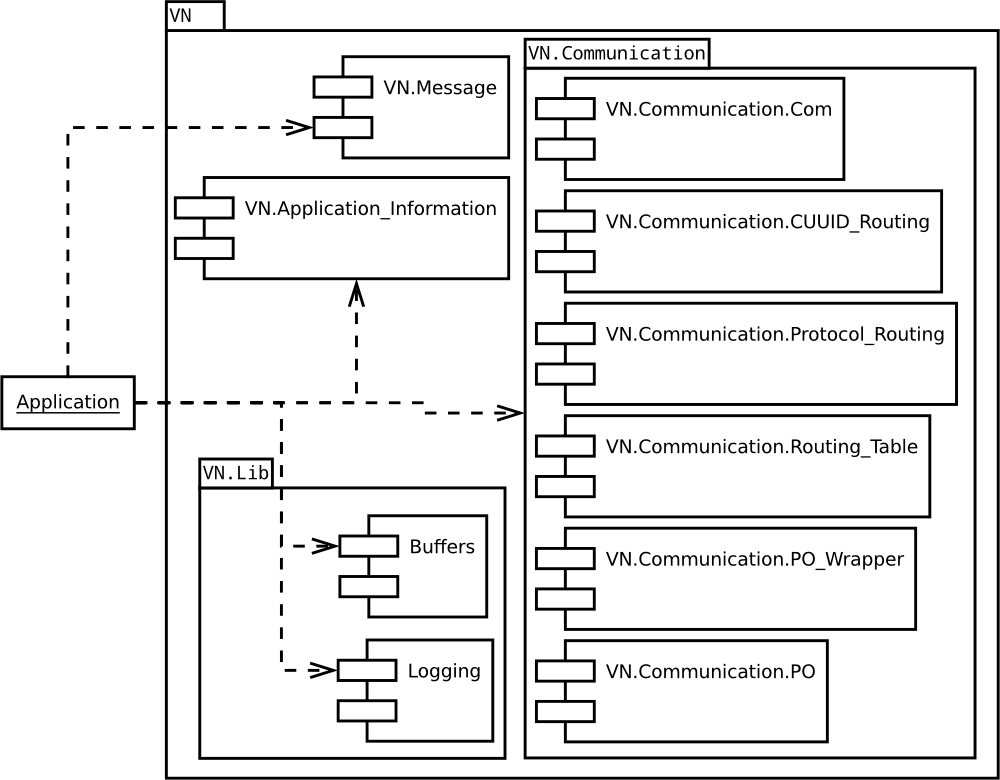
\includegraphics[width=\textwidth]{figures/appendix_component_overview}
    \caption{Component overview of the Virtual Network Library implementation.}
    \label{fig:appendix_component_overview}
\end{figure}

To get one simple application up and running in a "Virtual Network" the
application's settings need to be defined in the \emph{Application\_Information}
component. This range from everything from CUUID to other custom settings that
may be needed. The Application\_Information component also keeps track of the
application's logical address during run-time and supplies different helper
functions, one of which is to fill in \emph{VN.Message} header information.

The next step is to add connectivity. If the application only runs on a
processing node or another single subnet all that is needed is a
\emph{VN.Communication.Com} implementation of that specific subnet type. The
more advanced use case is a subnet manager that manages its own subnet and is
connected to a Local Subnet Manager on the processing node it runs on. As this
requires connectivty on more than one subnet a \emph{Protocol\_Routing} object
will be needed to route traffic between subnets. The Protocol\_Routing object
is a composite type of the VN.Communication.Com interface and can
therefore add multiple subnets during startup procedures.

All communication on a processing node through Ada Protected Objects goes
through the Subnet Manager as a router. This leads to that all applications on
a processing node only has to instantiate one connection. This is done by first
instantiating one Protocted Object (PO) through the \emph{VN.Communication.PO}
component. An access to this PO can then be used as input paramter when
creating the two \emph{VN.Communication.PO\_Wrapper's}, one for the application
and one for the local subnet manager.

The application itself is written as an Ada task and due to Ravenscar
limitiation must be built from the ground up for each new task. Best way to
start is to copy an example task from the "examples" directory in the
repository \cite{web:github-vn-lib}.

\section{Component and Service discovery process}\label{sec:discovery_process}
The following sequence diagrams show the basic component and service discovery
process for a local subnet using UDP/IP for inter-process communication
described in SPA Local Subnet Adaptation Draft \cite{spa:local-subnet}.

Figure
\ref{fig:appendix_vn_discovery_overview} starts with the high-level view of a
complete SPA network. Figure
\ref{fig:appendix_vn_local_subnet_network_discovery} continues with the
specifics of a SPA Local Subnet. Figure
\ref{fig:appendix_vn_address_block_assignment} shows the specifics on how a SPA
Subnet Manager aquires an address block from the CAS and after that the SPA
Subnet Manager assigns a logical address to each component it is aware of in
figure \ref{fig:appendix_vn_local_subnet_address_assignment}. The last step is the
component capabilities discovery process where the LS collects
information about all known components on the network, this is shown in figure
\ref{fig:appendix_vn_component_capabilities_discovery}.

\begin{figure}[h]
    \centering
    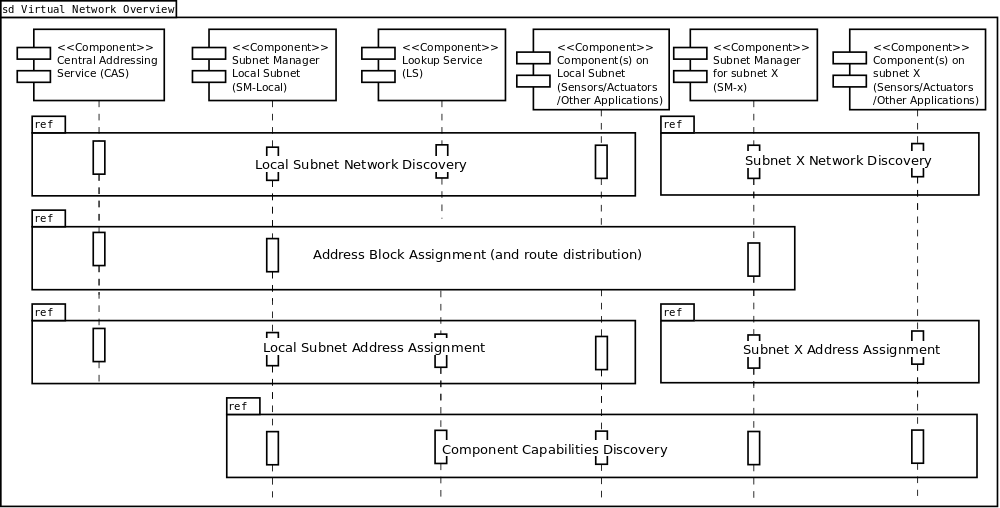
\includegraphics[width=\textwidth]{figures/vn_discovery_overview}
    \caption{Overview of the discovery process for a SPA network.}
    \label{fig:appendix_vn_discovery_overview}
\end{figure}

\begin{figure}[h]
    \centering
    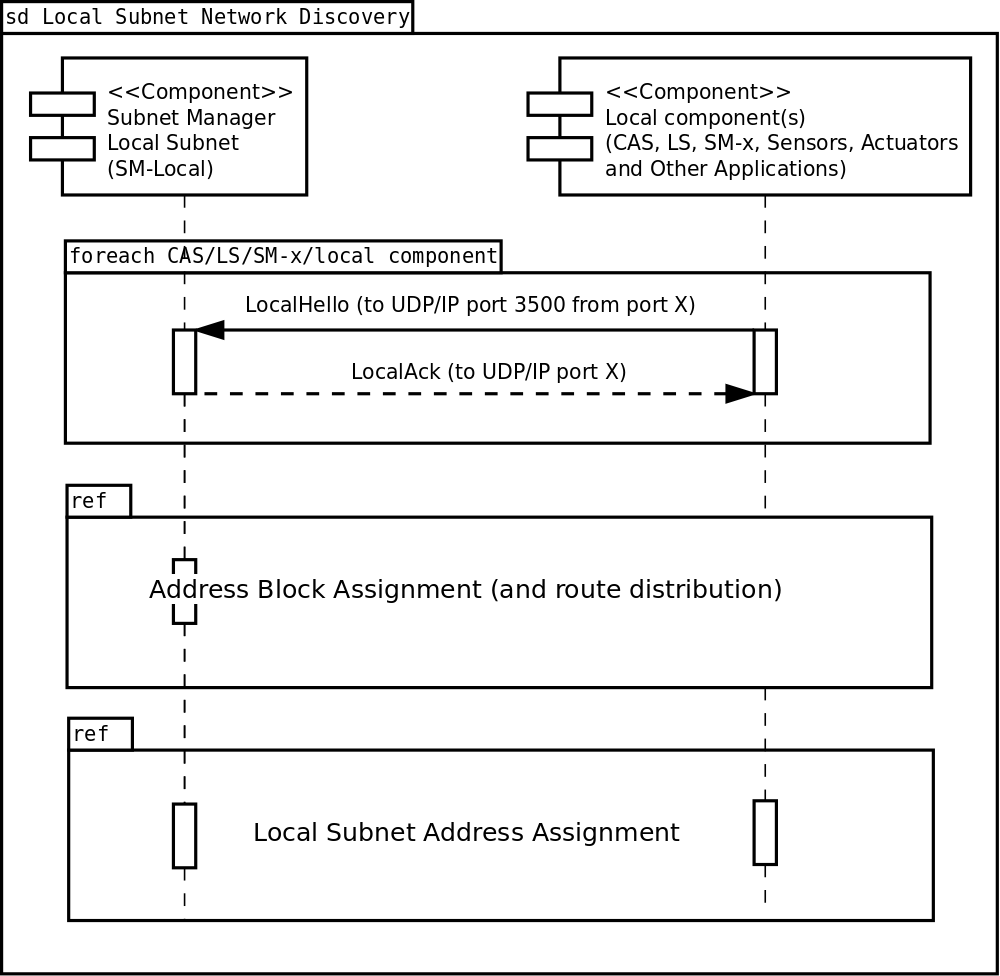
\includegraphics[width=\textwidth]{figures/vn_local_subnet_network_discovery}
    \caption{The basic discovery process for a SPA Local Subnet Discovery.}
    \label{fig:appendix_vn_local_subnet_network_discovery}
\end{figure}

\begin{figure}[h]
    \centering
    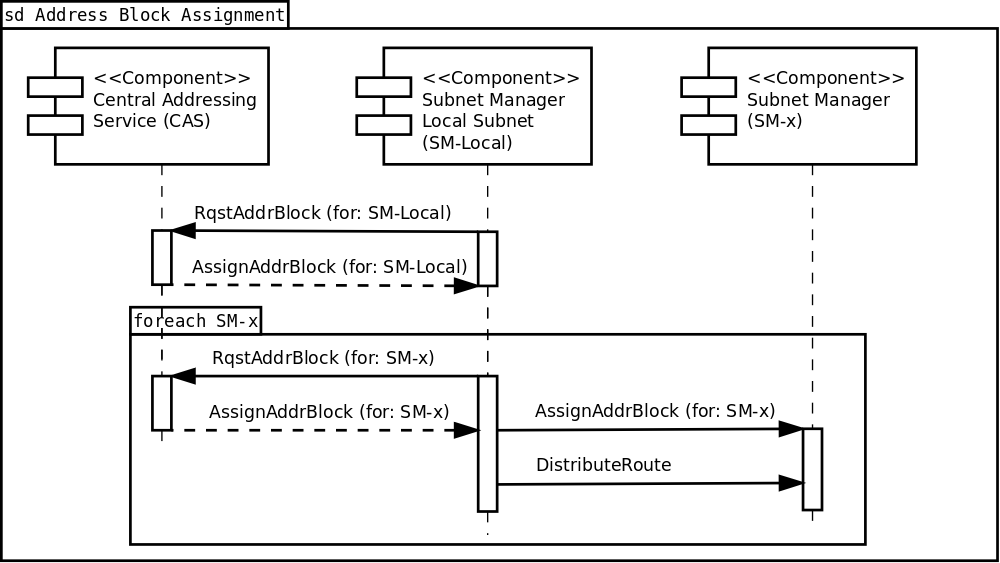
\includegraphics[width=\textwidth]{figures/vn_address_block_assignment}
    \caption{How the local subnet manager aquires address block from the CAS
    for its own subnet and for other connected subnet managers.}
    \label{fig:appendix_vn_address_block_assignment}
\end{figure}

\begin{figure}[h]
    \centering
    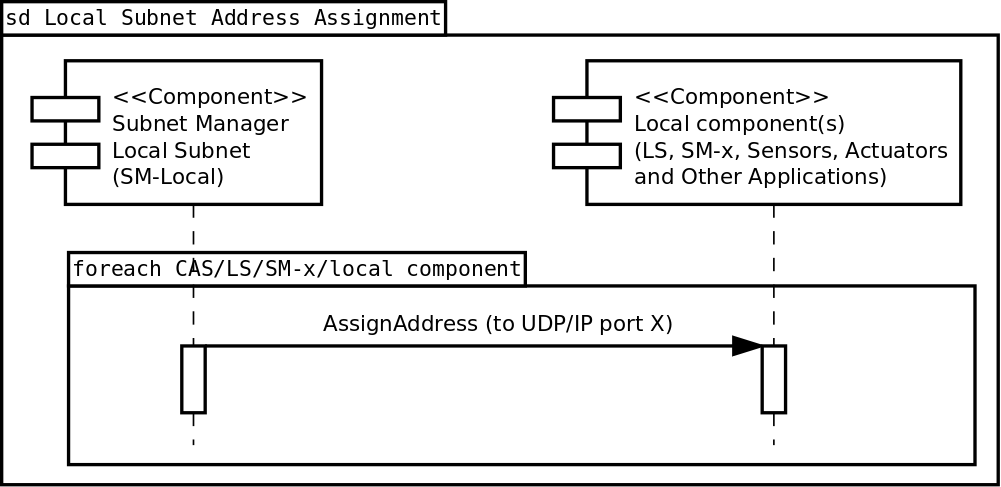
\includegraphics[width=\textwidth]{figures/vn_local_subnet_address_assignment}
    \caption{After the SM-L has received Address Block it starts to assign
    logical addresses to local components it's aware of.}
    \label{fig:appendix_vn_local_subnet_address_assignment}
\end{figure}

\begin{figure}[h]
    \centering
    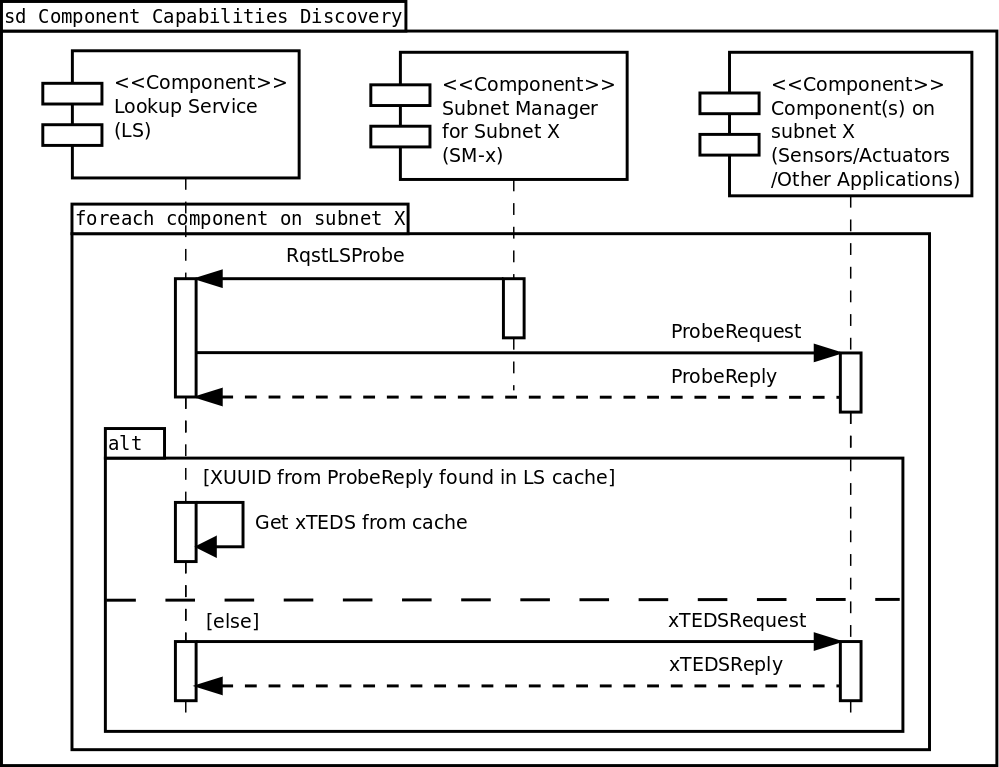
\includegraphics[width=\textwidth]{figures/vn_component_capabilities_discovery}
    \caption{The last step in the discovery process is to discovery which
    components have which services, capabilities that is.}
    \label{fig:appendix_vn_component_capabilities_discovery}
\end{figure}
